\chapter{Results and evaluation}
\label{chap:ResultsAndEvaluation}
The results are created with the Netherlands data set. A detailed model of the Netherlands would be around 24.1 GB. This is too large to load in too GPU memory. The whole tree is around 55 GB in size. This tree consist about 2200 nodes of different sizes and has a depth around 12. The test PC has 8 GB of CPU memory and 1 GB of GPU memory.

\section{Image results}
\label{sec:ImageResults}
Figure \ref{fig:UniversityCampus} shows an overview of the TU/e campus. This is a basic view of the campus. The river dommel is also shown through the campus. This picture is taken above the train tracks.

\begin{figure}[htb!]
\centering
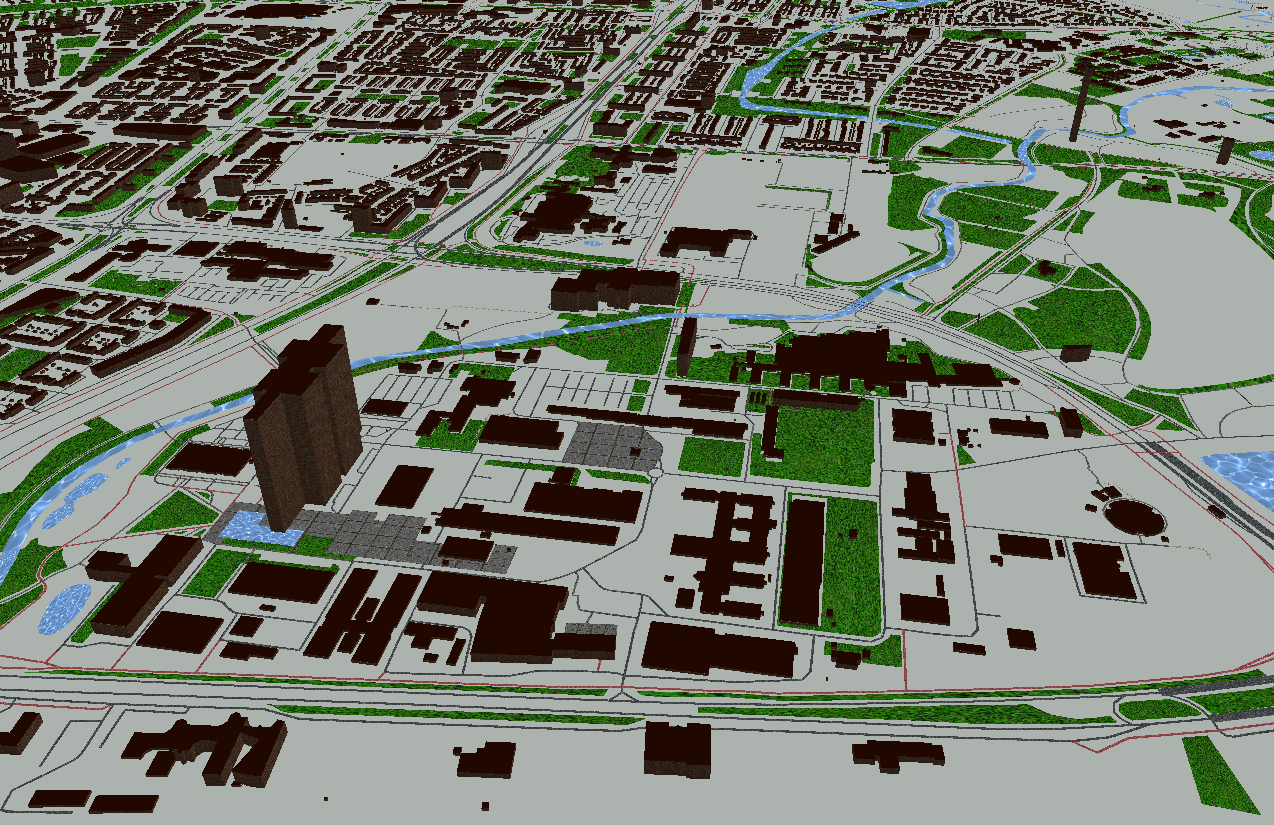
\includegraphics[width=\textwidth]{TUe}
\caption{University campus}
\label{fig:UniversityCampus}
\end{figure}

The error that is introduced when rendering from a distance is visible in figure \ref{fig:Simplification}. The top image is rendered with less error than the bottom version. In the simplified version, it is possible to see that the building is only a convex hull of its original. Also the roads that are besides the building are removed.

\begin{figure}[htb!]
\centering
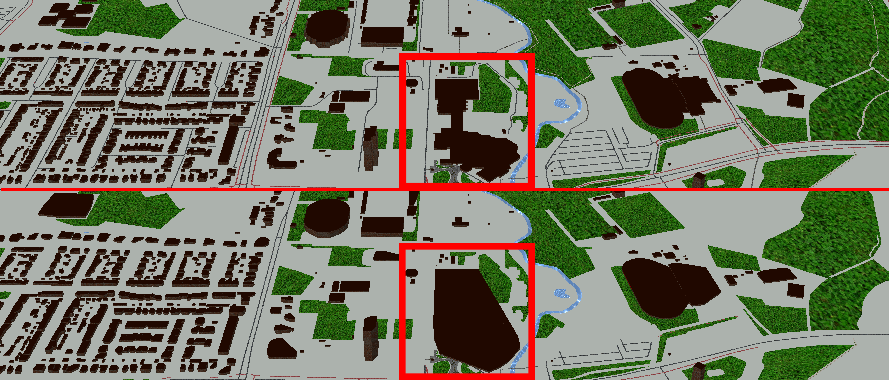
\includegraphics[width=\textwidth]{Simplification}
\caption{Top: detailed version, Bottom: Simplified version}
\label{fig:Simplification}
\end{figure}

\section{GPU usage}
\label{sec:GPUUsage}
We have tested the system with 2 different error settings. The blue is with a 10 000 error per meter and a maximum error of 10 000 000. This means the largest distance loaded is 1 KM. The red is with a 100 000 error per meter and a maximum error of 1 000 000 000. This means the largest distance loaded is 10 KM.

In graph \ref{graph:MemoryUsage} we see that the memory usage for the blue error setting is far lower and not really dependent on the position. When red error setting is used the system is a bit more position dependent and uses a lot more memory, but can still be hold in the GPU memory. In graph \ref{graph:DistanceGraph} the distance is lower than the maximum distances for the specified setting. Note that this is the fartest node, but the closest distance to that node. Notice that the distance is almost 10 folded for both city's, while only doubling the memory usage.

\begin{figure}[htb!]
\centering
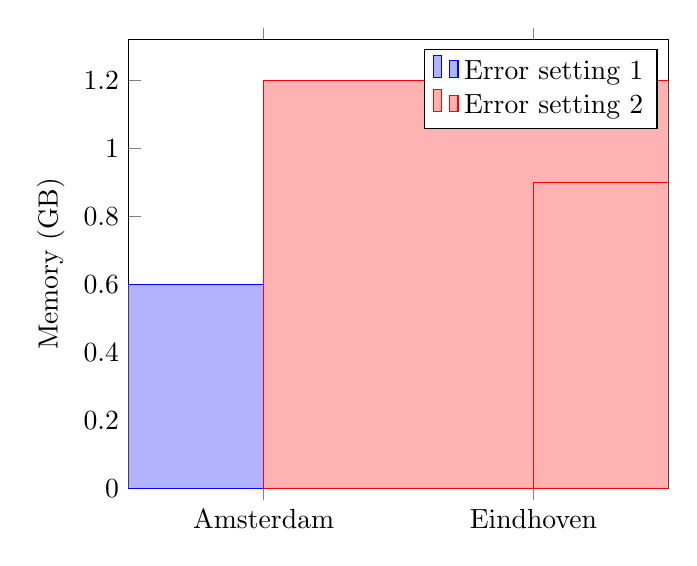
\begin{tikzpicture}
\begin{axis}[
    xtick={1,2},
    xticklabels={Amsterdam,
                Eindhoven},
    ybar=0pt,
    ymin=0,
    samples=2,
    domain=1:2,
    xtick=data,
    bar width=40,
    enlarge x limits={abs=0.5},
    ylabel={Memory (GB)}
]
        \addplot coordinates {
            (1,   0.6)
            (2,  0.6)
        };
        \addplot coordinates {
            (1,   1.2)
            (2,  0.9)
        };
        \legend{Error setting 1,Error setting 2}
\end{axis}
\end{tikzpicture}
\caption{Memory usage}
\label{graph:MemoryUsage}
\end{figure}

\begin{figure}[htb!]
\centering
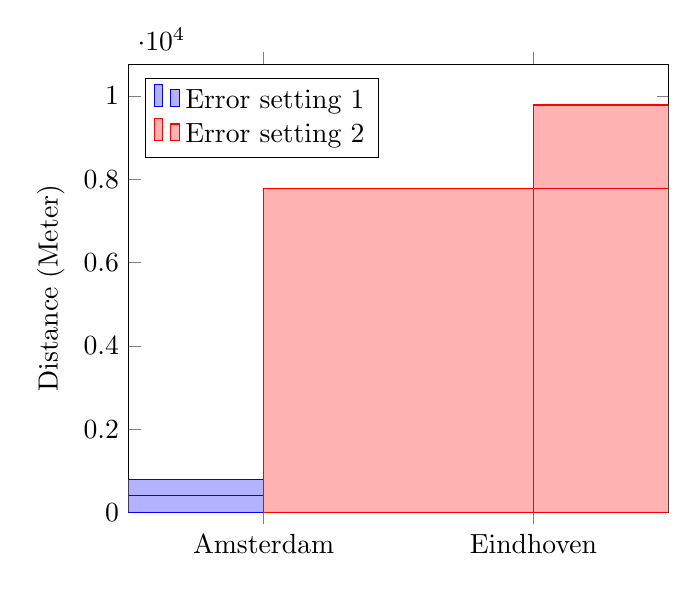
\begin{tikzpicture}
\begin{axis}[
    xtick={1,2},
    xticklabels={Amsterdam,
                Eindhoven},
    ybar=0pt,
    ymin=0,
    samples=2,
    domain=1:2,
    xtick=data,
    bar width=40,
    enlarge x limits={abs=0.5},
    ylabel={Distance (Meter)},
    legend pos=north west
]
        \addplot coordinates {
            (1,   407.557)
            (2,  797.977)
        };
        \addplot coordinates {
            (1,   7780.801)
            (2,  9786.661)
        };
        \legend{Error setting 1,Error setting 2}
\end{axis}
\end{tikzpicture}
\caption{Distance to furthest node}
\label{graph:DistanceGraph}
\end{figure}

\section{Limitations}
\label{sec:Limitations}
The height of buildings is determined with the building surface area of the building. If the building has an underground structure like underground parking garage, then the building is extremely high. The surface area of the geographic polygon is very small against the surface area of the whole building. This limitation expresses itself by generating very high building, while in reality the building above the ground is very low.

The width of a road is also approximated, by using meta-data. Sometimes this metadata isn’t available or wrong, which results in a different width. Also the road could have wider or smaller lanes.

